\section{Introduction}
%%%%%%%%%%%% MID WAY AGENDA %%%%%%%%%%%%%%
% \begin{frame}<beamer>
% \frametitle{Daniel Bähner Andersen}
% \tableofcontents[currentsection]
% \end{frame}	
%%%%%%%%%%%% MID WAY AGENDA %%%%%%%%%%%%%%

\begin{frame}{Introduction}{}
    \begin{itemize}            
	\item<1-> Water distribution network
	    \begin{itemize}  
			\item<1-> Necessary infrastructure 
			\item<1-> High energy consumption 
		\end{itemize}   
\end{itemize}
\begin{itemize}	
	\item<2-> Possible solution 
	\begin{itemize}	
		\item<2-> Introduction of water tower
		\item<2-> Advance control that ensure satisfying performance
	\end{itemize}
\end{itemize}
\begin{itemize}	
		\item<3-> \textit{How can a water tower be implemented in a water distribution network and controlled to minimize the cost of running the distribution network without violating constraints and compromising the water quality.}
    \end{itemize}           
\end{frame}



\begin{frame}{System description}{System description}

\begin{itemize}            
	\item<1-> 1:20 downscaled version of real water distribution system
\end{itemize} 
\vspace{-0.5cm}
\begin{figure}[H]
	\centering
	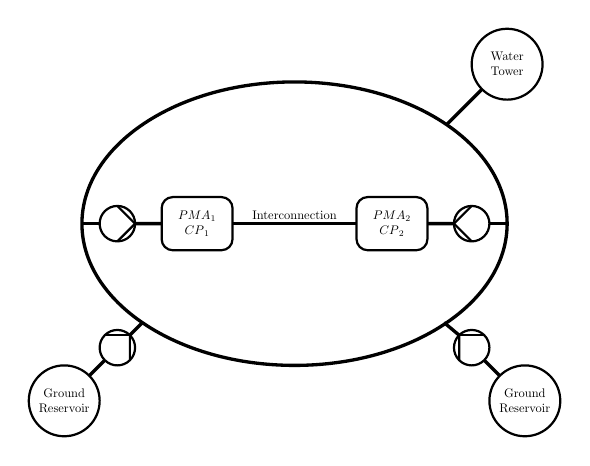
\begin{tikzpicture}[scale=0.45,transform shape]
\tikzstyle{box} = [draw,thick,rounded corners, minimum height=15mm, minimum width=20mm, align=center, text centered]
%Main Ring
\draw[very thick] (7,5.5) ellipse (6 and 4);
%Pump
\draw[thick,transform shape] (2,5.5) circle (0.5);
\draw[thick,transform shape] (2.5,5.5) -- (2,6);
\draw[thick,transform shape] (2.5,5.5) -- (2,5);
%Pump
\begin{scope} [rotate around={180:(12,5.5)}]
\draw[thick,transform shape] (12,5.5) circle (0.5);
\draw[thick,transform shape] (12.5,5.5) -- (12,6);
\draw[thick,transform shape] (12.5,5.5) -- (12,5);
\end{scope}
%Pump
\begin{scope} [rotate around={135:(12,2)}]
\draw[thick,transform shape] (12,2) circle (0.5);
\draw[thick,transform shape] (12.5,2) -- (12,2.5);
\draw[thick,transform shape] (12.5,2) -- (12,1.5);
\end{scope}
%Pump
\begin{scope} [rotate around={45:(2,2)}]
\draw[thick,transform shape] (2,2) circle (0.5);
\draw[thick,transform shape] (2.5,2) -- (2,2.5);
\draw[thick,transform shape] (2.5,2) -- (2,1.5);
\end{scope}
%Reservoirs
\node[thick,draw,circle,minimum width=20mm,align=center] (R1) at (0.5,0.5) {Ground \\ Reservoir};
\node[thick,draw,circle,minimum width=20mm,align=center] (ER1) at (13,10) {Water \\ Tower};
\node[thick,draw,circle,minimum width=20mm,align=center] (R2) at (13.5,0.5) {Ground \\ Reservoir};
%PMA and interconnection
\node[box] (PMA1) at (4.25,5.5) {$\text{PMA}_1$ \\ $\text{CP}_1$};
\node[box] (PMA2) at (9.75,5.5) {$\text{PMA}_2$ \\ $\text{CP}_2$};
\draw[very thick](PMA1) -- (PMA2);
\node[align=center] (PMAc) at (7,5.75) {Interconnection};
%Connections
\draw[very thick](1.2,1.2) -- (1.65,1.65);
\draw[very thick](2.34,2.34) -- (2.71,2.71);
\draw[very thick](12.8,1.2) -- (12.36,1.64);
\draw[very thick](11.66,2.34) -- (11.22,2.71);
\draw[very thick](13,5.5) -- (12.5,5.5);
\draw[very thick](11.5,5.5) -- (PMA2);
\draw[very thick](1,5.5) -- (1.5,5.5);
\draw[very thick](2.5,5.5) -- (PMA1);
\draw[very thick](12.28,9.28) -- (11.29,8.29);
\end{tikzpicture} 
\end{figure}\vspace{-0.5cm}
\end{frame}

\section{Modelling}
\subsection{Hydraulic Modelling}

\begin{frame}{Modelling}{Hydraulic Modelling}
\begin{itemize}
	\item<1-> Two-terminal components 
	\begin{itemize}
		\item<1-> Pipes 
		\item<1-> Pumps
		\item<1-> Valves
		\item<1-> Water tower
	\end{itemize}
	\item<1-> Modelled as pressure drop across each component
\end{itemize}

	\begin{itemize}
		\item<2-> Complete component model
	\end{itemize}
\onslide<2->{
\begin{equation}
\label{CompleteModel}
\Delta p_k = \underbrace{\lambda_k (q_k) + \zeta_k + J_k \dot{q_k}}_\text{Pipe} + \underbrace{\mu_k (q_k, OD)}_\text{Valve} - \underbrace{\alpha_k(\omega_k,q_k)}_\text{Pump} + \underbrace{\Delta p_{wt,k}}_\text{Water tower}
\end{equation}}

\end{frame}

\subsection{Graph representation}

\begin{frame}{Modelling}{Graph representation}
\begin{itemize}
	\item<1-> A mathematical way for representing a network
	\item<1-> Pressure drops across nodes
	\item<1-> Kirchhoff's Laws 
\end{itemize}
\vspace{-0.5cm}
\onslide<1->{
\begin{figure}[H]
\centering
\resizebox{0.75\linewidth}{!}{
%\usepackage {tikz}
%\usepackage{rotating}
%\usepackage{amsmath}
%\usetikzlibrary {positioning}


%\usepackage {xcolor}
%\begin{turn}{90}
\begin{tikzpicture}[-latex ,auto ,node distance =4 cm and 8cm ,
semithick , state/.style ={ draw,shape=circle}]

\node[circle,fill,inner sep=3pt,label=below right:$n_4$] (A) at (0,0) {};
\node[circle,fill,inner sep=3pt,label=right:$n_8$] (B) at (0,4) {};
\node[circle,fill,inner sep=3pt,label=below right:$n_9$] (C) at (0,8) {};
\path (A) edge  node[right] {$e_9 c_{18}$} (B);
\path (B) edge  node[right] {$e_{10}c_{19}$} (C);
\node[circle,fill,inner sep=3pt,label=right:$n_{10}$] (G) at (2,11) {};
\node[circle,fill,inner sep=3pt,label=right:$n_{11}$] (H) at (-1,10) {};
\node[circle,fill,inner sep=3pt,label=right:$n_{12}$] (I) at (-1,12) {};
\path (C) edge  node[right] {$e_{14}c_{23}$} (G);
\path (C) edge  node[right] {$e_{11}c_{22}$} (H);
\path (H) edge  node[right] {$e_{12}c_{21}$} (I);



%
\node[circle,fill,inner sep=3pt,label=below right:$n_5$] (D) at (8,0) {};
\node[circle,fill,inner sep=3pt,label=right:$n_{13}$] (E) at (8,4) {};
\node[circle,fill,inner sep=3pt,label=right:$n_{14}$] (F) at (8,8) {};
\path (D) edge  node[right] {$e_{16}c_{25}$} (E);
\path (E) edge  node[right] {$e_{17}c_{26}$} (F);
\node[circle,fill,inner sep=3pt,label=right:$n_{15}$] (J) at (9,11) {};
\node[circle,fill,inner sep=3pt,label=right:$n_{16}$] (K) at (7,10) {};
\node[circle,fill,inner sep=3pt,label=right:$n_{17}$] (L) at (6,12) {};
\path (F) edge  node[right] {$e_{21}c_{30}$} (J);
\path (F) edge  node[left] {$e_{18}c_{29}$} (K);
\path (K) edge  node[left] {$e_{19}c_{28}$} (L);

\node[circle,fill,inner sep=3pt,label=above:$n_{1}$] (M) at (4,14) {};

\path (A) edge  node[below] {$e_4 c_{9;10}$} (D);
\path (C) edge  node[below] {$e_{23}c_{42}$} (F);
\path (G) edge [bend right = -15] node[below left =0.15 cm] {$e_{15}c_{24}$} (M);
\path (L) edge [bend left = -15] node[below left =0.15 cm] {$e_{20}c_{27}$} (M);
\path (I) edge [bend right = -15] node[below =0.15 cm] {$e_{13}c_{20}$} (M);
\path (J) edge [bend left = -15] node[below =0.15 cm] {$e_{22}c_{31}$} (M);


\node[circle,fill,inner sep=3pt,label=above right :$n_{3}$] (N) at (-3,0) {};
\node[circle,fill,inner sep=3pt,label= above right:$n_{2}$] (O) at (-8,2) {};
\node[circle,fill,inner sep=3pt,label= above left :$n_{18}$] (P) at (-4,6) {};

\path (N) edge  node[below] {$e_3 c_8$} (A);
\path (P) edge [bend right = -50] node[below left =0.15 cm] {$e_{25}c_{33}$} (M);
\path (M) edge [bend left = -50] node[below =0.15 cm] {$e_1c_2$} (O);
\path (O) edge  node[below] {$e_2c_4$} (N);
\path (N) edge  node[right] {$e_{24}c_{32}$} (P);



\node[circle,fill,inner sep=3pt,label=above right:$n_{6}$] (Q) at (11,0) {};
\node[circle,fill,inner sep=3pt,label=above right :$n_{7}$] (R) at (14,6) {};
\path (Q) edge  node[below] {$e_5 c_{11}$} (D);
\path (R) edge  node[below right ] {$e_7 c_{14}$} (Q);
\path (M) edge [bend right = -40] node[below =0.15 cm] {$e_8 c_{16}$} (R);
\path (Q) edge [bend right = -20] node[below =0.15 cm] {$e_6 c_{12;13}$} (N);


\end{tikzpicture}
%\end{turn}
%\end{sidewaysfigure}
}
\end{figure}
}

\end{frame}


\begin{frame}{Modelling}{Graph representation}
\begin{itemize}
	\item<1-> A mathematical way for representing a network
	\item<1-> Pressure drops across nodes
	\item<1-> Kirchhoff's Laws 
\end{itemize}
\vspace{-0.5cm}
\onslide<1->{
\begin{figure}[H]
\centering
\resizebox{0.75\linewidth}{!}{
%\usepackage {tikz}
%\usepackage{rotating}
%\usepackage{amsmath}
%\usetikzlibrary {positioning}


%\usepackage {xcolor}
%\begin{turn}{90}
\begin{tikzpicture}[-latex ,auto ,node distance =4 cm and 8cm ,on grid ,
semithick ,
state/.style ={ draw,shape=circle}]

\node[circle,fill,inner sep=3pt,label=below right:$n_4$] (A) at (0,0) {};
\node[circle,fill,inner sep=3pt,label=right:$n_8$] (B) at (0,4) {};
\node[circle,fill,inner sep=3pt,label=below right:$n_9$] (C) at (0,8) {};
\path (A) edge  node[right] {$e_9 c_{18}$} (B);
\path (B) edge  node[right] {$e_{10}c_{19}$} (C);
\node[circle,fill,inner sep=3pt,label=right:$n_{10}$] (G) at (2,11) {};
\node[circle,fill,inner sep=3pt,label=right:$n_{11}$] (H) at (-1,10) {};
\node[circle,fill,inner sep=3pt,label=right:$n_{12}$] (I) at (-1,12) {};
\path (C) edge  node[right] {$e_{14}c_{23}$} (G);
\path (H) edge  node[right] {$e_{12}c_{21}$} (I);



%
\node[circle,fill,inner sep=3pt,label=below right:$n_5$] (D) at (8,0) {};
\node[circle,fill,inner sep=3pt,label=right:$n_{13}$] (E) at (8,4) {};
\node[circle,fill,inner sep=3pt,label=right:$n_{14}$] (F) at (8,8) {};
\path (D) edge  node[right] {$e_{16}c_{25}$} (E);
\path (E) edge  node[right] {$e_{17}c_{26}$} (F);
\node[circle,fill,inner sep=3pt,label=right:$n_{15}$] (J) at (9,11) {};
\node[circle,fill,inner sep=3pt,label=right:$n_{16}$] (K) at (7,10) {};
\node[circle,fill,inner sep=3pt,label=right:$n_{17}$] (L) at (6,12) {};
\path (F) edge  node[left] {$e_{18}c_{29}$} (K);
\path (K) edge  node[left] {$e_{19}c_{28}$} (L);

\node[circle,fill,inner sep=3pt,label=above:$n_{1}$] (M) at (4,14) {};

\path (G) edge [bend right = -15] node[below left =0.15 cm] {$e_{15}c_{24}$} (M);
\path (L) edge [bend left = -15] node[below left =0.15 cm] {$e_{20}c_{27}$} (M);
\path (I) edge [bend right = -15] node[below =0.15 cm] {$e_{13}c_{20}$} (M);
\path (J) edge [bend left = -15] node[below =0.15 cm] {$e_{22}c_{31}$} (M);


\node[circle,fill,inner sep=3pt,label=above right :$n_{3}$] (N) at (-3,0) {};
\node[circle,fill,inner sep=3pt,label= above right:$n_{2}$] (O) at (-8,2) {};
\node[circle,fill,inner sep=3pt,label= above left :$n_{18}$] (P) at (-4,6) {};

\path (P) edge [bend right = -50] node[below left =0.15 cm] {$e_{25}c_{33}$} (M);
\path (M) edge [bend left = -50] node[below =0.15 cm] {$e_1c_2$} (O);
\path (N) edge  node[right] {$e_{24}c_{32}$} (P);



\node[circle,fill,inner sep=3pt,label=above right:$n_{6}$] (Q) at (11,0) {};
\node[circle,fill,inner sep=3pt,label=above right :$n_{7}$] (R) at (14,6) {};
\path (R) edge  node[below right ] {$e_7 c_{14}$} (Q);
\path (M) edge [bend right = -40] node[below =0.15 cm] {$e_8 c_{16}$} (R);


\end{tikzpicture}
%\end{turn}
%\end{sidewaysfigure}
}
\end{figure}
}

\end{frame}




